\documentclass[a4paper,12pt]{article}

\input{"$HOME/Desktop/Studia/LaTeX/setup.tex"}



\author{Wojciech Orłowski}
\title{Dyskretny rozkład Bernouliego - sprawozdanie}

\begin{document}
    \maketitle

    \section{Wstęp}

    Jednym z często używanych rozkładów dyskretnych jest rozkład Bernouliego.
    Zmienną dyskretną Bernouliego nazywamy taką zmienną losową, która może przyjmować dwie wartości.
    Wartości te mogą oznaczać sukces w doświadczeniu (z prawdopodobieństwem $p$) lub jego porażkę (z prawdopodobieństwem $1 - p$). 
    Niech zmienna ta przyjmuje wartość 1, jeżeli wynikiem jest sukces oraz 0, jeżeli wynikiem jest porażka.
    \[f(0) = P\{ Y = 0 \}  = 1 - p \; \; \text{oraz} \; \; 
        f(1) = P\{ Y = 1 \}  = p.\]
    W prosty sposób można wyznaczyć wartość oczekiwaną i wariancję tej zmiennej losowej, w zależności od prawdopodobieństwa $p$
    \[ E[Y] = 0(1-p) + 1p = p, \]
    \[ Var(Y) = E[Y^2] - E[Y]^2 = p - p^2 = p(1-p). \]  
    Korzystając z ogólnodostępnego rozkładu jednorodnego możemy w prosty sposób skonstruować zmienną Bernouliego.
    Dla liczby wylosowanej z jednorodnym prawdopodobieństwem z przedziału [0,1] wynik doświadczenia Bernouliego (z prawdopodobieństwem $p$) uznajemy za sukces, jeżeli wylosowana liczba jest mniejsza niż $p$.
    Przy skończonej liczbie doświadczeń Bernouliego wartość oczekiwaną możemy wyestymować za pomocą średniej arytmetycznej wyników
    \[ E[Y] = \frac{1}{N} \sum_{i = 1}^{N} Y_i, \]
    gdzie $Y_i$ oznacza wynik $i$-tego doświadczenia.

    \section{Cel}

    Celem ćwiczenia jest zapoznanie z generowaniem liczb o rozkładzie Bernouliego.
    Ponadto porównano estymowane wartości wartości oczekiwanej oraz wariancji z obliczonymi analitycznie.
    Wartości te zostały wyznaczone dla różnej liczby generowanych doświadczeń.

    \newpage

    \section{Wyniki}

    Obliczenia zostały wykonane w języku \julia, który jest przeznaczony dla obliczeń numerycznych,~a~także stochastycznych.
    Wygenerowane zostały wartości oczekiwane i wariancji dla maksymalnie $N= 10^7$ eksperymentów Bernouliego.
    Na wykresy zostały naniesione błędy względne dla $n = \{10^2, 10^3, 10^4, 10^5, 10^6, 10^7\}$.
    Błędy względne zostały obliczone za pomocą 
    \[ \text{błąd względny} = \frac{\abs{\text{wartość estymowana} - \text{wartość analityczna}}}{\text{wartość analityczna}}. \]
    Wyznaczone wartości oczekiwane oraz wariancje zostały przedstawione na rys. \ref{fig:rys}.
    \begin{figure}[h]
        \centering
        \begin{subfigure}{0.49\textwidth}
            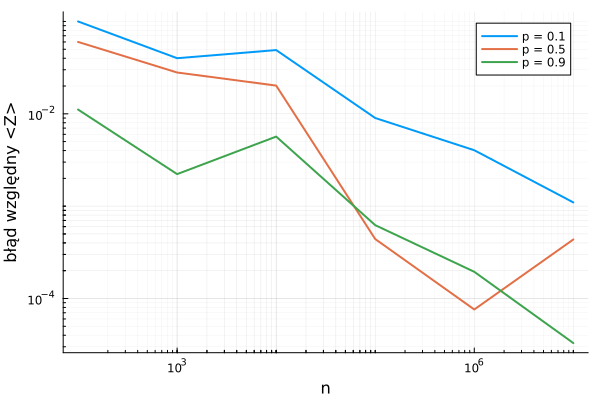
\includegraphics[width = \textwidth]{../galeria/rel_err_exp_val.png}
            \caption{}
        \end{subfigure}
        \begin{subfigure}{0.49\textwidth}
            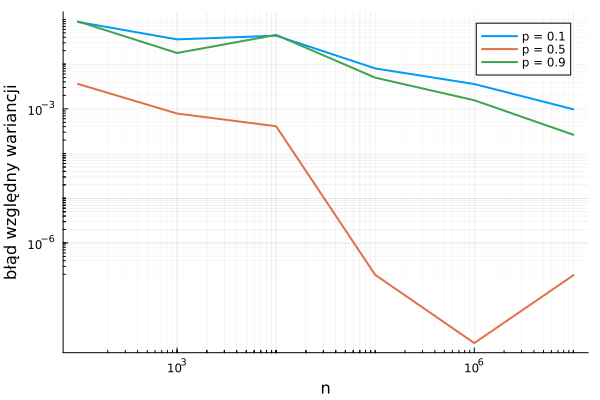
\includegraphics[width = \textwidth]{../galeria/rel_err_var.png}
            \caption{}
        \end{subfigure}
        \caption{(a) Błąd względny wartości oczekiwanej, (b) błąd względny wariancji.}
        \label{fig:rys}
    \end{figure}
    Jak można zauważyć błąd względny maleje wraz z ilością wykonanych doświadczeń Bernouliego, to znaczy wygenerowanych liczb. 
    Warto jednak zaznaczyć, że nawet dla wysoko zoptymalizowanego języka programowania taka ilość operacji jest znacząca i wymaga dokładnego przemyślenia obliczeń.
    Należy zaplanować małą liczbę alokacji pamięci oraz jak najmniejszą liczbę zapisywanych danych.
    Ponadto obliczenia można znacznie przyspieszyć licząc wariancje i wartość oczekiwaną w jednej pętli, zliczając sumę i sumę kwadratów wylosowanych zmiennych.
    Przykładowo obliczając wariancję i wartość oczekiwaną przy każdym losowaniu nowej zmiennej wszystkie obliczenia trwają (zgodnie z procedurą @\texttt{time} języka Julia)
    \begin{verbatim}
        16.017455 seconds (450.00 M allocations: 7.153 GiB, 3.47% gc time).
    \end{verbatim}
    Natomiast dla obliczania wariancji i odchylenia tylko 6 razy podczas $10^7$ losowań obliczenia trwają tylko
    \begin{verbatim}
        9.670301 seconds (240.00 M allocations: 4.023 GiB, 3.57% gc time),
    \end{verbatim}
    mimo, że wymaga to dodatkowo sprawdzenia warunku, czy przy danym losowaniu wykonać obliczenia. 
    Ważne jest zatem rozważne przeprowadzanie tego typu eksperymentów stochastycznych, gdyż większa liczba losowań oraz nieprzemyślany algorytm długi czas trwania symulacji i dużą liczbę niepotrzebnych alokacji pamięci.

    \newpage

    \section{Podsumowanie}

    W krótkim ćwiczeniu udało się przeanalizować wpływ ilości przeprowadzanych losowań na dokładność oszacowania wariancji i wartości oczekiwanej.
    Można zauważyć, że dla większej liczby losowań ogólnie błąd względny jest mniejszy. 
    Ponadto przeanalizowano wpływ przemyślanego algorytmu na czas obliczeń.
    Przy doświadczeniach stochastycznych, gdzie wykonywana jest raczej duża liczba losowań i operacji ważnym jest, aby kod i algorytm był przemyślany i zoptymalizowany.


\end{document}
